%\subsection{Quadrillage}
\SbSSCT{Quadrillage}{Grid}


\begin{tabular}{|c|}\hline 
\tikz \draw(0,0) grid (2,2); 
\\ \hline 
\BS{draw} (0,0) \RDD{grid} (2,2); \RRR{14-8}
\\ \hline 
\end{tabular} 


\bigskip
\begin{tabular}{|c|c|c|c|} \hline 
\multicolumn{4}{|c|}{ \BS{draw} (0,0) grid  [\RDD{step}=.75cm] (0,0) grid (3,3);   }\\ 
\hline  
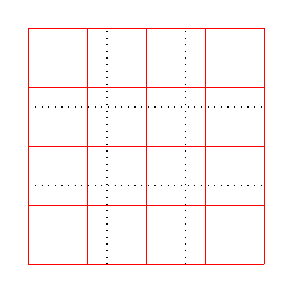
\begin{tikzpicture}
\draw[dotted](0,0) grid (3,3); 
%\draw[thick] (0,0) grid [step=1] (3,2);
\draw[red] (0,0) grid [step=.75cm] (3,3);
\end{tikzpicture}
&  
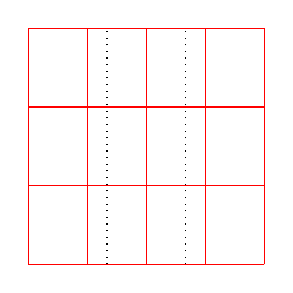
\begin{tikzpicture}
\draw[dotted](0,0) grid (3,3); 
%\draw[thick] (0,0) grid [step=1] (3,2);
\draw[red] (0,0) grid [xstep=.75cm] (3,3);
\end{tikzpicture}
&  
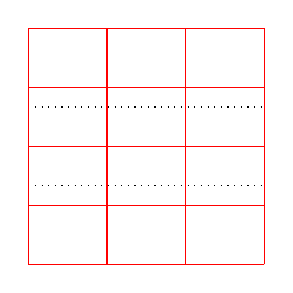
\begin{tikzpicture}
\draw[dotted](0,0) grid (3,3); 
%\draw[thick] (0,0) grid [step=1] (3,2);
\draw[red] (0,0) grid [ystep=.75cm] (3,3);
\end{tikzpicture}
&
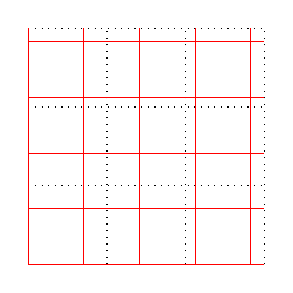
\begin{tikzpicture}
\draw[dotted](0,0) grid (3,3); 
%\draw[thick] (0,0) grid [step=1] (3,2);
\draw[red] (0,0) grid [step=(45:1)] (3,3);
\end{tikzpicture}
\\ \hline 
step=.75cm & x step=.75cm & ystep=.75cm  & step=(45:1)
\\ \hline 
\end{tabular} 

\bigskip

\begin{tabular}{|c|c|} \hline 
 
\BS{draw}[red] (0,0) grid [\RDD{rotate}=45] (3,3);
&  
\BS{draw}[\RDD{help lines}] (0,0) grid  (3,3);
\\ \hline  
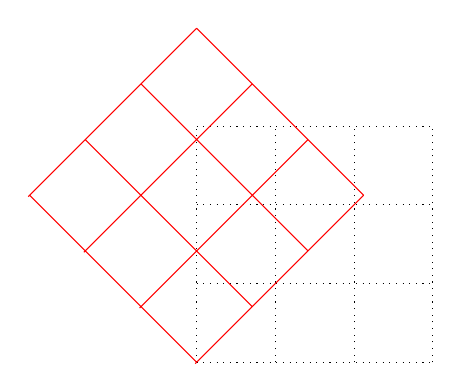
\begin{tikzpicture}
\draw[dotted](0,0) grid (3,3); 
%\draw[thick] (0,0) grid [step=1] (3,2);
\draw[red] (0,0) grid [rotate=45] (3,3);
\end{tikzpicture}
& 
\tikz \draw[help lines] (0,0) grid (3,3); \\ 
\hline 
\end{tabular} 



%\begin{tabular}{|c|c|c|c|c|} \hline 
%\multicolumn{5}{|c|}{ \BS{tikz} \BS{draw} [\RDD{step}=1mm] (0,0) grid (2,2);   }\\ 
%\hline  
%\tikz \draw[step=1mm] (0,0) grid (2,2);
%&  
%\tikz[rotate=30] \draw (0,0) grid (2,2);
%&  
%\tikz \draw (0,0) grid [xstep=.5] (2,2);
%&  
%\tikz \draw (0,0) grid [ystep=.5] (2,2);
%&
%\tikz \draw[help lines] (0,0) grid (2,2);
%\\ \hline  
%[\RDD{step}=1mm] & [\RDD{rotate}=30] & [\RDD{xstep}=.5] & [\RDD{ystep}=.5] & [\RDD{help lines}] \\ 
%\hline 
%\end{tabular} 
